\section{Input}

\subsection{Medium Selection}
\label{sec:medium-selection}

The first step in this project was to establish the best method for a student to interact with the application. As seen in \cref{sec:previous-works} different mediums for OMR have been tried, however which one would be most suitable for a student to use wouldn't necessarily correlate with which was best for quality of scanning, speed of analysis etc.

\subsubsection{Flat Bed Scanner}

The most simple of all the input methods, this would involve a student writing on a sheet of manuscript paper, then using a flat bed scanner (the type commonly found as a standalone device and in multi-function printers) to input the sheet into the computer. This method allows for a scan with high and consistent light levels (minimising noise and light-dependent artefacts), minimal distortion due to paper curvature (as the scanner usually flattens the sheet) and a high resolution end image, typically 300-600dpi.

The application would process the sheet using traditional OMR techniques and then provide feedback to the student. This technique would therefore require ownership of both a scanner and a computer on which to install and run the application. Alternatively, the student could upload the scanned image to a web based service for analysis, removing the need to install software.
%
%\subsubsection{Photograph/Camera}
%
%\todo[inline,color=red]{Implementation - Photo/Camera}
%
%Total free for all, colours and light levels vary, extraction from background, resolution variable, noise variable
%
%Reference `Project 8 Final Report'

\subsubsection{Gestures}\label{sec:gestures}

Taking input on a tablet enables the capturing of individual strokes. I decided to leverage more traditional OMR techniques by first rendering the strokes as an image but there is potential for future research to see if using statistical features of the strokes themselves in a similar way to the methods described by \cite{taubman2005musichand} and \cite{george2003online}. I also looked as character recognition using multi-stroke gestures and \$ N-Stroke recognisers and variations such as \$ N-Protractor in \cite{anthony2012n}.

My main reason for not investigating gesture based recognition further at present is that the recognition techniques seemed to rely on users having a consistent stroke structure for the different note entities. The most promising work is that of \cite{taubman2005musichand} but even then, the project used a very rigid structure of which entities were expected to be drawn in which order.

There also seemed to be a small number of users in the \cite{taubman2005musichand} study and the author notes that user testing and experiments on the transferability of models between users was not done. Sadly I can't preform a lengthly calibration stage where I can trust the user's input which makes a per-user model difficult.

\subsubsection{Tablet Input}

Although I decided not to use tablet gestures directly, I did opt to use a tablet as my primary method of input.

In testing it proved a fairly natural experience for the children who trailed \noteED using the freedrawing environment. Interestingly both finger and stylus work well as input methods and although I didn't gather data on the quality of drawing versus the input method, there were no immediate differences of problems encountered by using one over the other for children.

Interesting, adults seemed to prefer the stylus, my hypothesis for this (which was then confirmed in further conversation) was that since adults have larger fingers, it's harder for them to accurately track the point at which their line is being drawn on the canvas.

\begin{figure}[h!]
    \centering
    \begin{subfigure}[b]{.49\linewidth}
        \centering
        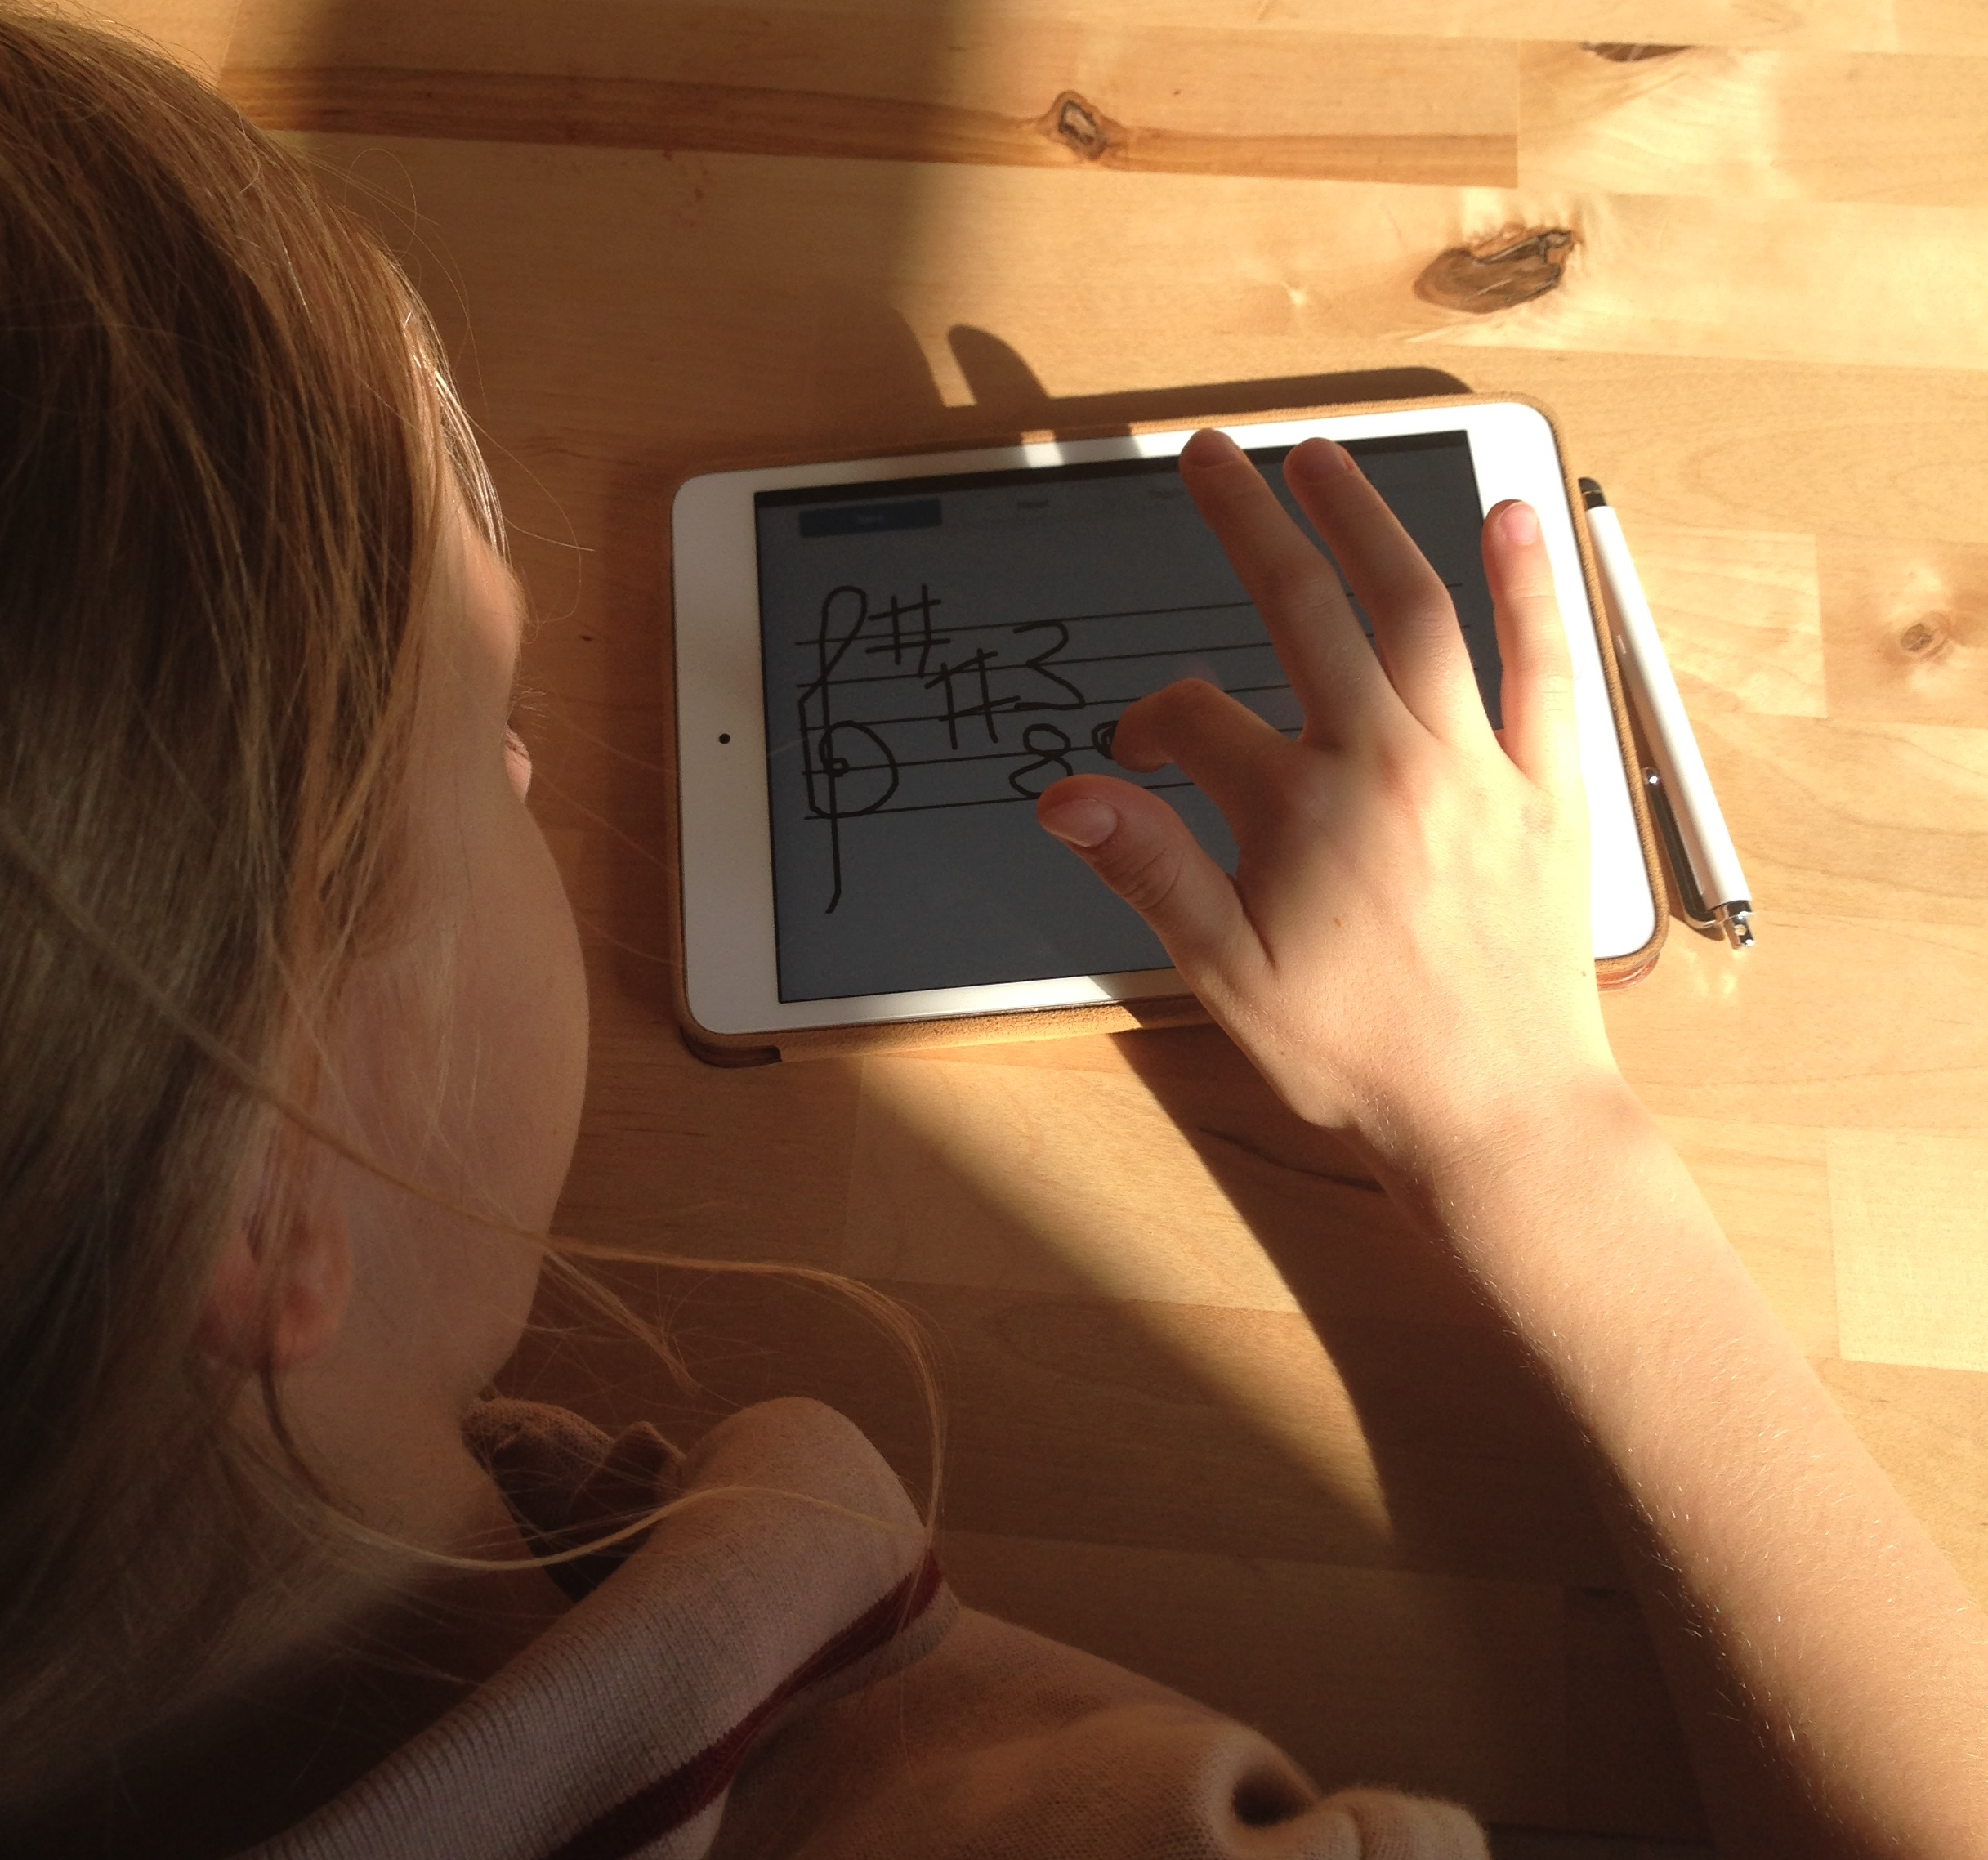
\includegraphics[width=\linewidth]{gfx/photos/user-finger.jpg}
        \caption{Using a finger}
    \end{subfigure}
    \begin{subfigure}[b]{.49\linewidth}
        \centering
        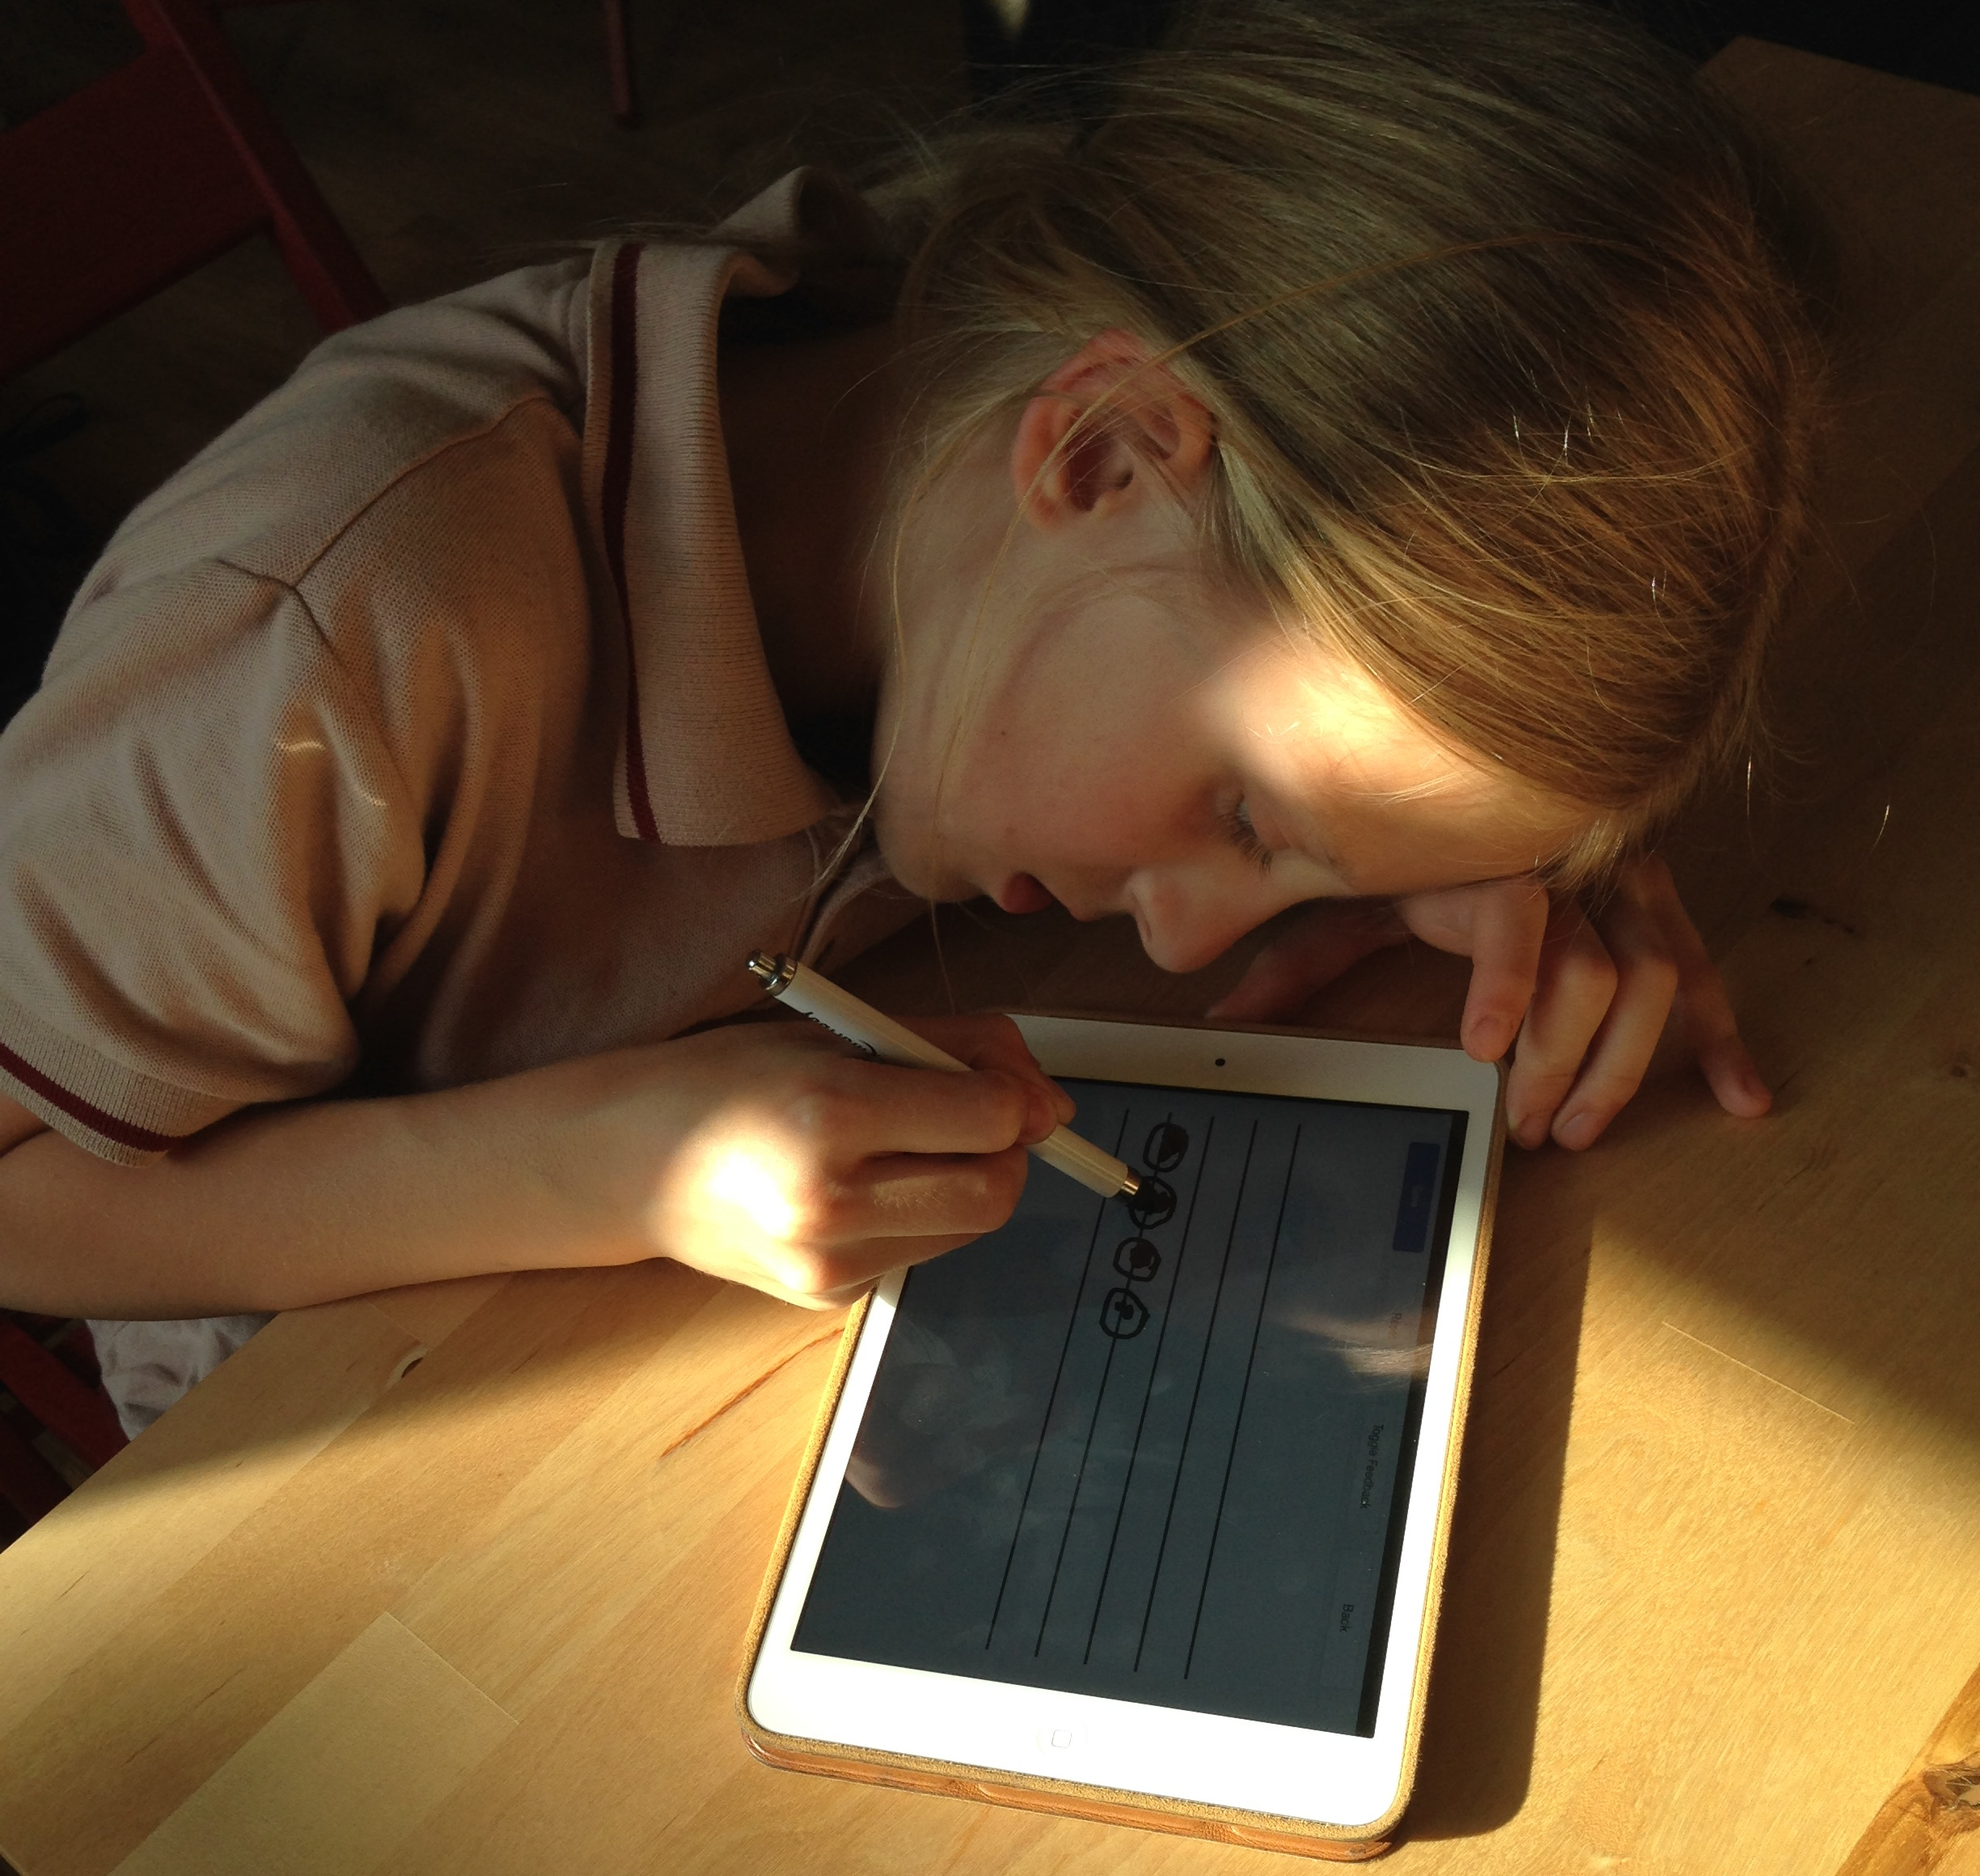
\includegraphics[width=\linewidth]{gfx/photos/user-stylus.jpg}
        \caption{Using a stylus}
    \end{subfigure}

    \caption{Examples of a student trying different tablet input methods}
\end{figure}

It was also suggested to me that if the application could be accessed through a web browser and scale according to the browser, many schools now have smartboards\footnote{http://smarttech.com/Home+Page/Solutions/Education+Solutions/Products+for+education} which are in effect large tablets.

\subsection{Capturing Strokes}
\label{sec:capturing-strokes}
To capture strokes drawn by the user, several listeners are attached to the HTML5 canvas element on which the manuscript is rendered. When the user presses their mouse down or initiates a touch event, a new array of line points is created and the initial point of interaction is stored in that array. From there, any mouse or touch movement whilst the touch or `mousedown' event is active triggers a new point recording, until the mouse button is released or the touch event ends. In this way, an array of points is built up which represent a drawn line.

Each time the line changes via the addition of new points, a redraw event is triggered which connects all the points together and renders the line onto the canvas.

In initial experiments with simple manuscript entities, this worked well, however as children began to experiment with more complex entities (requiring more lines and therefore more points) the length of time required to redraw the lines on the canvas became prohibitively long. Eventually a lag occurred between `pen' movement and lines being rendering on the canvas, the result of which was that as more lines were drawn, the time between new points being registered increased. This increase led to the drawing experience feeling (as one user described it) `really clunky' and long straight lines appearing instead of smooth curves (\cref{fig:drawing-lag-rough}).

\begin{figure}[hbt                                   ]
    \centering

    \begin{subfigure}[b]{.49\linewidth}
        \centering
      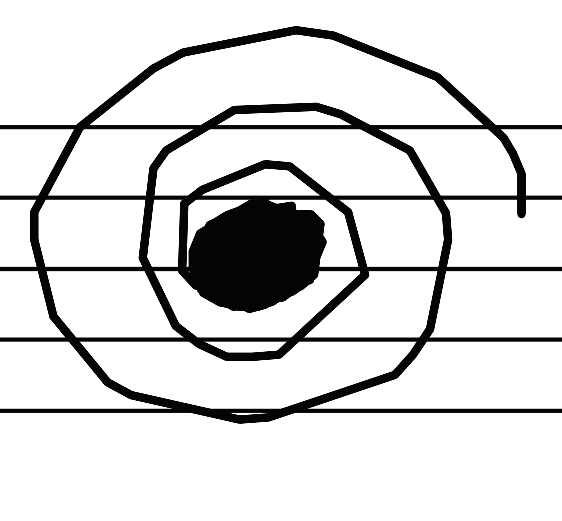
\includegraphics[width=\linewidth]{gfx/implementation/lag-stave.png}
      \caption{Drawing with refresh rendering - note that after drawing a high density region of many points, a spiral outward is very `angular' due to the additional time it takes to redraw so many points on every movement event }
      \label{fig:drawing-lag-rough}
    \end{subfigure}
    \begin{subfigure}[b]{.49\linewidth}
        \centering
      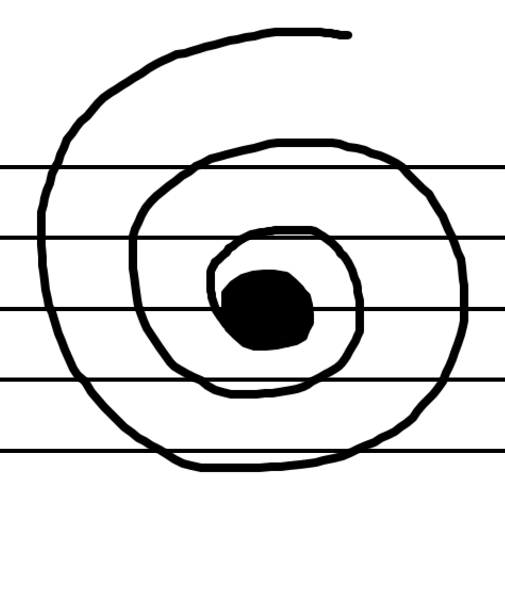
\includegraphics[width=\linewidth]{gfx/implementation/nolag-stave.png}
      \caption{Drawing with incremental rendering, not that after a similar high density region of points, the curve outwards still appears smooth}
      \label{fig:drawing-lag-smooth}
    \end{subfigure}

  \label{Drawing Lag}

\end{figure}

To counteract this, I modified the code such that it renders new line segments on the fly, rather than re-rendering all the lines every time a new point is added. Although this requires some more logic to render the line segment, overall the experience turned out much smoother as the small increase in the length of the code path had much less impact than re-rendering the drawing every time (\cref{fig:drawing-lag-smooth}).

\section{Data Storage and Retrieval}

\subsection{Stave Drawing}
I store the data gathered in \cref{sec:capturing-strokes} in two ways.

Firstly, I store the serialised JSON of the stroke data in the database which is postiive for several reasons pertaining to future work as well as immediate benefits for \noteED. It enables more potential experiments in future in the area of gesture based segmentation and recognition (see \cref{sec:gestures}) and could support showing a student corrections by transforming points in the strokes as opposed to transformations on the image. It also facilitates some great UI features like playing back the drawing for the tutor so they can see exactly how the student approached the problem.

Secondly, I store the entire rendered canvas in the cloud using an Amazon S3 bucket, as a `reference copy' in case I need to check the JSON against the original image at a later date or re-analyse images after updating my classifiers, features or analysis techniques.

\subsection{Components}

Once components have been extracted from the drawing using the techniques outlined in \cref{sec:identification}, I store both their features and \acrfull{RLE} representation of the whole component in the database for retrieval later during any further image processing.

Although 3000 components uses around 1GB in data when raw, using compression we are able to lower this considerably using run length encoding as shown in \ref{table:rle-improvement}.

\begin{table}[H]

    \begin{tabularx}{\textwidth}{ X X X X }
    \toprule
    Metric                  & Without RLE   & With RLE   & Improvement \\
    \midrule
    Storage Required        & 759 MB        & 22 MB      & 91.7\%      \\
    Total Retrieval Time    & 1639 ms       & 42 ms      & 97.4\% \\
    \bottomrule
    \end{tabularx}

    \caption{To improve the speed of my application, I utilised \acrfull{RLE} (covered in \cref{sec:tb-rle}) to improve storage and retrieval times during feature extraction and classification by up to 97\% (\cref{table:rle-improvement}).}
    \label{table:rle-improvement}
\end{table}

\subsection{Database Schema}

\begin{table}[H]

    \begin{tabularx}{\textwidth}{ l l X }
      \toprule
      Column                 & Type                       \\
      \midrule
      id         & integer                     \\
      email      & character varying(255)      \\
      created\_at & timestamp without time zone \\
      updated\_at & timestamp without time zone \\
      \midrule
      \multicolumn{3}{c}{Indexes} \\
      \midrule
      users\_pkey & \multicolumn{2}{c}{PRIMARY KEY, btree (id)} \\
      \bottomrule
    \end{tabularx}

    \caption{Components Table}
    \label{table:db-components}
\end{table}

\begin{table}[H]

    \begin{tabularx}{\textwidth}{ l l X }
      \toprule
      Column           & Type                       \\
      \midrule
      id               & integer                     \\
      user\_id          & integer                     \\
      file             & character varying(255)      \\
      binary\_file\_data & bytea                       \\
      created\_at       & timestamp without time zone \\
      updated\_at       & timestamp without time zone \\
      json\_data        & json                        \\
      \midrule
      \multicolumn{3}{c}{Indexes} \\
      \midrule
      drawings\_pkey & \multicolumn{2}{c}{PRIMARY KEY, btree (id)} \\
      \bottomrule
    \end{tabularx}

    \caption{Drawings Table}
    \label{table:db-drawings}
\end{table}

\begin{table}[H]

    \begin{tabularx}{\textwidth}{ l l X }
      \toprule
      Column                 & Type                       \\
      \midrule
      id                    & integer                     \\
      drawing\_id           & integer                     \\
      features              & json                        \\
      created\_at           & timestamp without time zone \\
      updated\_at           & timestamp without time zone \\
      manual\_class         & character varying(255)      \\
      parent\_component\_id & integer                     \\
      auto\_class           & character varying(255)      \\
      feedback              & json                        \\
      \midrule
      \multicolumn{3}{c}{Indexes} \\
      \midrule
      components\_pkey & \multicolumn{2}{c}{PRIMARY KEY, btree (id)} \\
      \bottomrule
    \end{tabularx}

    \caption{Components Table}
    \label{table:db-components}
\end{table}

\subsection{Entity Relationship Diagram}

The following is a summarised view of the core entities that make up \noteED and how they're related to each other.

\begin{figure}[hbt]
  \centering
  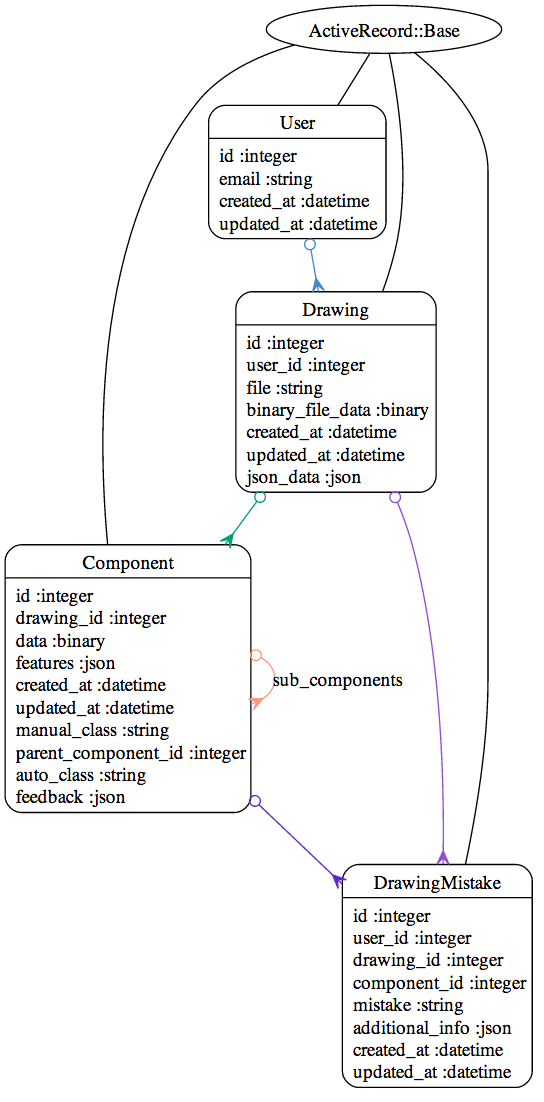
\includegraphics[width=.6\linewidth]{gfx/models-complete.png}
  \caption{\noteED Entity relationship diagram}
  \label{fig:erd}
\end{figure}





